\documentclass[../monografia.tex]{subfiles}
\graphicspath{ {images/}{../images/} } 

\begin{document}
% Detalhar neste item os procedimentos realizados para os testes de funcionamento dos sub-sistemas, da inter-relação dos subsistemas e do sistema completo.

\section{Resultados dos Testes}
\section{Verificação dos requisitos}




\begin{figure}[h]
	\centering
	\begin{subfigure}{0.5\textwidth}
		\centering
	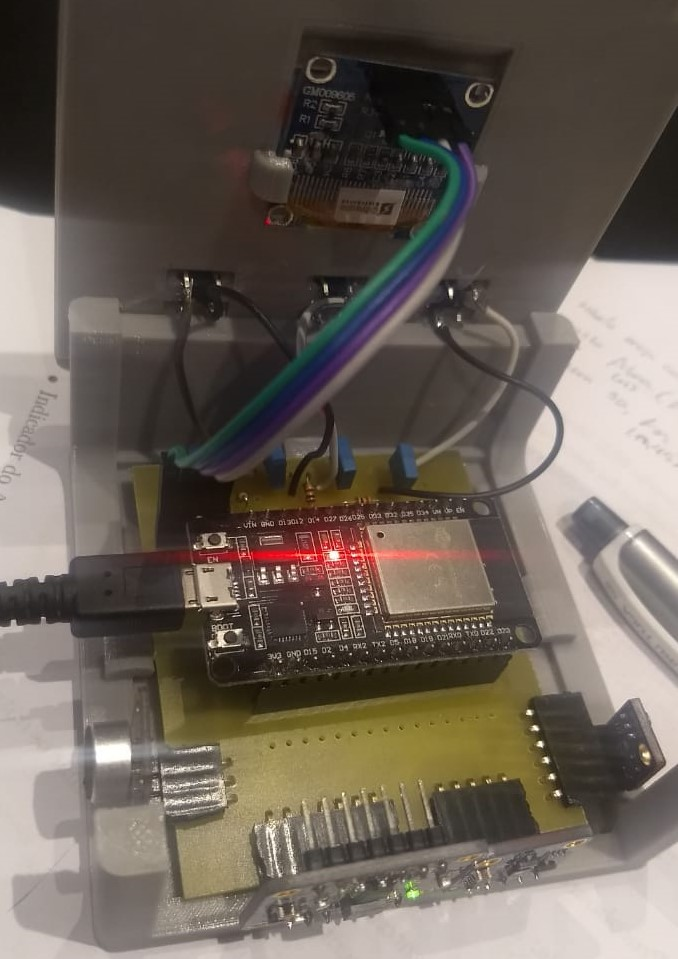
\includegraphics[width=0.8\textwidth]{placa-final}
	\caption{Interna}
	\label{fig:interna}
	\end{subfigure}%
	\begin{subfigure}{0.5\textwidth}
		\centering
		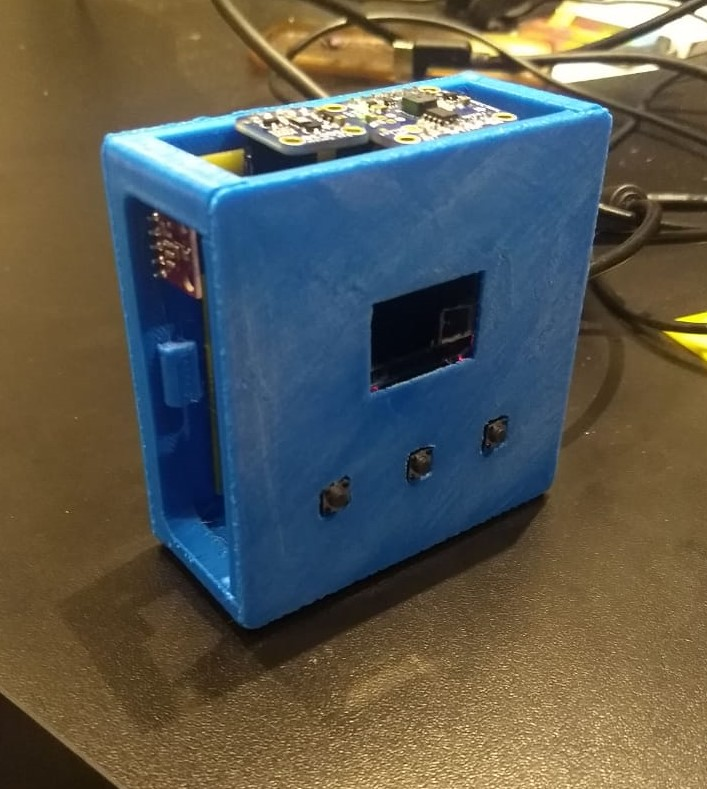
\includegraphics[width=\textwidth]{montagem-final.jpg}
		\caption{Externa}
		\label{fig:externa}
	\end{subfigure}
	\caption{Montagem final do dispositivo}
	\label{fig:mecanicas}
\end{figure}


\end{document}